% =============================================================================
% Block 8 --- Aula 8: AS-AD microfoundations (Benigno 2015, sections 1-5). Checks: practice-all-topics-check-b.py, Block 8.
% Solution format (rules/00_estilo_avaliacao.md §4): Notation list, numbered equations cited with \eqref,
% one operation per displayed line. Labels: b8:AD, b8:AS (notation paragraph), b8q<question>:<name>.
\bloco{8}{The New Keynesian AS--AD model: microfoundations}{Benigno (2015) \S\S1--5 (Aula 8) \,\textbullet\, 25 points}

{\footnotesize\noindent\textbf{Notation for Blocks 8--9 (Benigno 2015).} Lower-case letters are log deviations from an efficient
steady state; bars denote the long run. Households: $u(C)-v(L)+\beta\{u(\bar C)-v(\bar L)\}$, $u_c=C^{-1/\tilde\sigma}$, $v=L^{1+\eta}/(1+\eta)$,
$\rho\equiv-\ln\beta$; resources $y=s_cc+g$, $\sigma\equiv\tilde\sigma s_c$. Firms: technology $Y(j)=AL(j)$, desired markup $\mu$ (monopoly power and
taxes, $\mu\simeq\mu_\theta+\tau+\tau_c$, with $\tau$ collecting labor, payroll and sales taxes); a fraction $\alpha$ of prices is preset at $p^e$.
AD, Benigno's eq.~(21), and AS, eq.~(20), with $\kappa=\frac{(1-\alpha)(\sigma^{-1}+\eta)}{\alpha}$:
\begin{align}
y&=\bar y_n+(g-\bar g)-\sigma[i-(\bar p-p)-(\bar\tau_c-\tau_c)-\rho], \tag{AD}\label{b8:AD}\\
p-p^e&=\kappa(y-y_n). \tag{AS}\label{b8:AS}
\end{align}
Calibration when numbers are asked (Benigno, p.~515): $\alpha=0.66$, $\sigma=0.5$, $\eta=0.2$, so $\sigma^{-1}+\eta=2.2$, $\kappa=1.133$.\par}

\questao{(5 points) Objective items.}

\textbf{a)} (3 points) Why does Benigno's AD curve slope downward in the $(y,p)$ plane?
\begin{alternativas}
\item A higher $p$ lowers real balances $M/P$, so the interest rate that clears the money market rises and spending falls.
\item A higher $p$, given $\bar p$, raises expected inflation $\bar p-p$, which lowers the real rate and pushes households to consume.
\item A higher $p$ lowers real balances, so the central bank's money-supply rule raises $i$ and households save more today.
\item A higher $p$, given $i$ and $\bar p$, lowers expected inflation $\bar p-p$, so the real rate rises and households save more.
\end{alternativas}
\gabarito{D}
\begin{sol}
\begin{notacao}
\item $y$, $p$: output and price level; $\bar p$: long-run price level; $i$: nominal rate; $i-(\bar p-p)$: real rate; $\sigma>0$.
\end{notacao}
\passo{key}{Differentiating \eqref{b8:AD} with $i$ and $\bar p$ fixed:}
\begin{equation}
\frac{\partial y}{\partial p}=-\sigma. \label{b8q22:slope}
\end{equation}
$p\uparrow$ means $\bar p-p\downarrow$, so the real rate $i-(\bar p-p)$ rises and the Euler equation moves consumption from today to
tomorrow. The channel is intertemporal; there is no LM curve, because the instrument is $i$.
\passo{distractors}{A is the IS--LM (Keynes-effect) story. B gets the sign of $\bar p-p$ wrong, which would reverse the sign of
\eqref{b8q22:slope} and make the curve slope upward. C makes two mistakes: the money-market channel and a money-supply instrument the model does not have.}
\refbib{Benigno (2015), \S3, eqs.~(1)--(6), pp.~505--506, and \S5, eq.~(21), p.~509.}
\end{sol}

\medskip
\textbf{b)} (2 points, T or F) News that the long-run desired markup $\bar\mu$ will be higher (current $\mu$ unchanged) shifts the AS curve
up today, because firms that reset prices raise them in anticipation.
\gabarito{F}
\begin{sol}
\begin{notacao}
\item $y_n$, $\bar y_n$: natural output today and in the long run; $a$, $g$, $\mu$ and $\bar a$, $\bar g$, $\bar\mu$: productivity, spending and markup today and in the long run.
\end{notacao}
\passo{proof}{\eqref{b8:AS} depends on $p^e$ and on current natural output, Benigno's eq.~(15), which contains the current $\mu$ only:}
\begin{equation}
y_n=\frac{(1+\eta)a+\sigma^{-1}g-\mu}{\sigma^{-1}+\eta}. \label{b8q22:yn}
\end{equation}
$\bar\mu$ enters the long-run version of \eqref{b8q22:yn},
\begin{equation}
\bar y_n=\frac{(1+\eta)\bar a+\sigma^{-1}\bar g-\bar\mu}{\sigma^{-1}+\eta}, \label{b8q22:ybn}
\end{equation}
which is in \eqref{b8:AD}. Differentiating \eqref{b8q22:ybn}, $d\bar y_n=-\frac{d\bar\mu}{\sigma^{-1}+\eta}$: lower expected permanent income cuts
consumption today, so the \emph{AD} shifts left by $\frac{d\bar\mu}{\sigma^{-1}+\eta}$. Rule: barred variables move the AD; current markups and
productivity move the AS.
\refbib{Benigno (2015), \S4, eq.~(15), and \S5, eq.~(21), pp.~507--509; Prova~01, Q3(a).}
\end{sol}

% -----------------------------------------------------------------------------
\questao{(8 points) \textit{Source: built on Benigno, P. (2015), ``New-Keynesian Economics: An AS--AD View'', \S4.1--\S4.4,
pp.~507--509 --- the article has no exercises; the statement below is ours.}
Natural versus efficient output: Benigno's eqs.~(14)--(15) and (19), the topic of Lista~7 Q3. Set $g=0$.}

\noindent What the article states (p.~509): ``A comparison of (19) with (15) shows that productivity and public spending shift the two
definitions of output in equal proportion. Mark-up shocks, however, are a source of inefficiencies, as they shift the natural but not
the efficient level of output.''

\textbf{a)} (3 points) Derive natural output $y_n$ (flexible prices) and efficient output $y_e$ (planner), and the gap between them.
\resolespaco
\begin{sol}
\begin{notacao}
\item $P$, $W$: price and nominal wage; $w-p$: log real wage; $A$, $a=\ln A$: productivity; $\mu\ge0$: desired markup.
\item $L$, $l$: hours and their log; $C$, $c$: consumption and its log; $y$: log output; $g=0$.
\item $\eta>0$: inverse Frisch elasticity; $\tilde\sigma>0$: intertemporal elasticity; $\sigma=\tilde\sigma s_c$; $u_c$, $v_l$: marginal utility of consumption and disutility of work.
\item $y_n$: natural output (flexible prices, with the markup); $y_e$: efficient output (planner, no markup).
\end{notacao}
\passo{natural}{A flexible firm sets its price as a markup over marginal cost $W/A$:}
\begin{equation}
P=(1+\mu)\frac WA. \label{b8q23:price}
\end{equation}
In logs, with $\ln(1+\mu)\simeq\mu$, \eqref{b8q23:price} gives the real wage firms pay:
\begin{equation}
w-p=a-\mu. \label{b8q23:ld}
\end{equation}
Labor supply equates the marginal rate of substitution to the real wage:
\begin{equation}
\frac{v_l(L)}{u_c(C)}=\frac WP. \label{b8q23:ls}
\end{equation}
In logs, \eqref{b8q23:ls} is
\begin{equation}
w-p=\eta l+\tilde\sigma^{-1}c. \label{b8q23:lsl}
\end{equation}
Technology and resources give
\begin{equation}
l=y-a,\qquad \tilde\sigma^{-1}c=\sigma^{-1}(y-g)=\sigma^{-1}y. \label{b8q23:tech}
\end{equation}
Substitute \eqref{b8q23:tech} into \eqref{b8q23:lsl} and equate with \eqref{b8q23:ld}:
\begin{align}
\eta\,(y-a)+\big(\sigma^{-1}y\big)&=(a-\mu)\nonumber\\
(\sigma^{-1}+\eta)\,y&=(1+\eta)a-\mu\nonumber\\
y_n&=\frac{(1+\eta)a-\mu}{\sigma^{-1}+\eta}. \label{b8q23:yn}
\end{align}
\passo{efficient}{The planner solves}
\begin{equation}
\max_Y\ u(Y)-v(Y/A). \label{b8q23:plan}
\end{equation}
The first-order condition of \eqref{b8q23:plan} is
\begin{equation}
u_c=\frac{v_l}{A},\quad\text{i.e.}\quad \mathrm{MRS}=\frac{v_l}{u_c}=A, \label{b8q23:pfoc}
\end{equation}
the marginal product of labor. In logs, using \eqref{b8q23:tech}, \eqref{b8q23:pfoc} is the first line of \eqref{b8q23:yn} with $\mu=0$:
\begin{align}
\eta\,(y-a)+\big(\sigma^{-1}y\big)&=a-(0)\nonumber\\
\eta(y-a)+\sigma^{-1}y&=a\nonumber\\
y_e&=\frac{(1+\eta)a}{\sigma^{-1}+\eta}. \label{b8q23:ye}
\end{align}
\passo{gap}{Subtract \eqref{b8q23:ye} from \eqref{b8q23:yn}:}
\begin{align}
y_n-y_e&=\Big(\frac{(1+\eta)a-\mu}{\sigma^{-1}+\eta}\Big)-\Big(\frac{(1+\eta)a}{\sigma^{-1}+\eta}\Big)\nonumber\\
&=-\frac{\mu}{\sigma^{-1}+\eta}<0. \label{b8q23:gap}
\end{align}
The markup is a wedge between the real wage firms pay ($A/(1+\mu)$, by \eqref{b8q23:price}) and the marginal product ($A$), so the
market works too little.
\rubrica{\item $y_n$ derived: 1.5 pts; $y_e$ derived: 1 pt; gap: 0.5 pt. Formulas quoted without derivation: max.\ 1 pt.}
\end{sol}

\textbf{b)} (3 points) Draw the labor market in the plane (hours $l$, real wage $w-p$) with $a=0$, marking natural and efficient
hours, and shade the welfare loss. Compute $y_n-y_e$ and the loss for $\mu=5\%$ at the calibration.
\resolespaco
\begin{sol}
\begin{notacao}
\item Symbols as in (a); $l_n$, $l_e$: natural and efficient hours (logs), with $a=0$.
\end{notacao}
\passo{graph}{With $a=0$, \eqref{b8q23:tech} gives $y=l$, so labor supply \eqref{b8q23:lsl} becomes}
\begin{align}
w-p&=\eta\,(l)+\sigma^{-1}(l)\nonumber\\
&=(\sigma^{-1}+\eta)\,l, \label{b8q23:sup}
\end{align}
with slope 2.2. The planner's line is $w-p=0$ (the marginal product); the market's line is $w-p=-\mu$, by \eqref{b8q23:ld}.
Setting \eqref{b8q23:sup} equal to each line:
\begin{align}
(\sigma^{-1}+\eta)\,l_n&=(-\mu),\qquad (\sigma^{-1}+\eta)\,l_e=(0),\nonumber\\
l_n&=-\frac{\mu}{\sigma^{-1}+\eta},\qquad l_e=0. \label{b8q23:ln}
\end{align}
\begin{center}
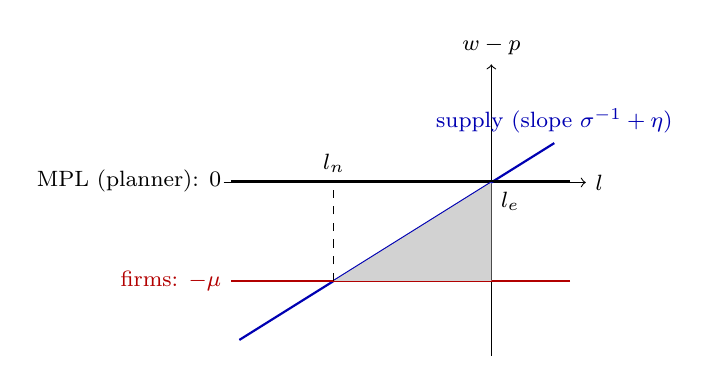
\begin{tikzpicture}[scale=1]
\draw[->] (-3.4,0) -- (1.2,0) node[right] {\footnotesize $l$};
\draw[->] (0,-2.2) -- (0,1.5) node[above] {\footnotesize $w-p$};
\draw[thick,blue!70!black] (-3.2,-2.0) -- (0.8,0.5) node[above] {\footnotesize supply (slope $\sigma^{-1}+\eta$)};
\draw[thick,red!70!black] (1.0,-1.25) -- (-3.3,-1.25) node[left] {\footnotesize firms: $-\mu$};
\draw[thick,black] (1.0,0.02) -- (-3.3,0.02) node[left] {\footnotesize MPL (planner): $0$};
\fill[gray!35] (-2.0,-1.25) -- (0,0) -- (0,-1.25) -- cycle;
\draw[dashed] (-2.0,-1.25) -- (-2.0,0) node[above] {\footnotesize $l_n$};
\node[below right] at (0,0) {\footnotesize $l_e$};
\end{tikzpicture}
\end{center}
\passo{numbers}{With $a=0$, $y=l$, so by \eqref{b8q23:ln}}
\begin{align*}
y_n-y_e&=l_n-l_e\\
&=\Big(-\frac{0.05}{2.2}\Big)-(0)\\
&=-2.27\%,
\end{align*}
as \eqref{b8q23:gap} also gives. The shaded triangle is the surplus lost on the hours not worked: its height is the wedge $\mu$
and its base is $l_e-l_n$ from \eqref{b8q23:ln}, so
\begin{align*}
\text{loss}&=\tfrac12\cdot\mu\cdot\frac{\mu}{\sigma^{-1}+\eta}\\
&=\tfrac12\cdot(0.05)\cdot\frac{(0.05)}{(2.2)}\\
&=\frac{0.05^2}{2\times2.2}=0.057\%\ \text{of output}.
\end{align*}
\refbib{Confirmed against the Lista~7 answer in \emph{Map}, \texttt{lista-07.md} ($-2.27\%$, $0.057\%$) and the instructor's key, PSET~7 Q4 ($y_n$ under flexible prices; $y_e$ removes market power).}
\rubrica{\item Graph: axes labeled, supply, the two horizontal lines, $l_n<l_e$: 1.5 pts. \item Numbers: 1.5 pts (gap 1, triangle 0.5).}
\end{sol}

\textbf{c)} (2 points) Which of $\alpha$, $\theta$, $a$, $g$ and the tax rates move $y_n-y_e$? Can monetary policy close it? What could?
\resolespaco
\begin{sol}
\begin{notacao}
\item $\theta>1$: elasticity of substitution between goods; $\mu_\theta=\ln\frac\theta{\theta-1}$: markup from monopoly power; $\alpha$: share of preset prices.
\end{notacao}
\passo{answer}{By \eqref{b8q23:gap}, only $\mu$ moves it: $\theta$ (via $\mu_\theta$) and the taxes in $\mu$. Productivity and spending move $y_n$ and $y_e$ by the
same amount (\eqref{b8q23:yn} and \eqref{b8q23:ye} have the same $a$ coefficient); stickiness $\alpha$ is in neither (they are flexible-price objects).
Monetary policy moves $y$ along \eqref{b8:AS}, not $y_n$, so it can make $y=y_e$ only by holding $p\neq p^e$. Closing the wedge itself
takes a real instrument: a production subsidy, financed lump sum, that offsets the markup (or lower distorting taxes).}
\rubrica{\item Correct list with the reason: 1 pt. \item Monetary vs fiscal instrument: 1 pt. ``Stickiness causes $y_n<y_e$'': 0 in the item.}
\end{sol}

% -----------------------------------------------------------------------------
\questao{(12 points) Discursive. \emph{Brazil's consumption-tax reform in the AS--AD model.} The reform replaces several taxes with
a value-added tax that phases in over years. Treat each fiscal change below as a deviation from an efficient steady state with
$p^e=\bar p=0$, $g=\bar g=0$ and $i=\rho$.}

\textbf{a)} (4 points) The household's budget is $(1+\tau_c)PC+\frac{(1+\bar\tau_c)\bar P\bar C}{1+i}=WL+\frac{\bar W\bar L}{1+i}+T$. Derive the Euler equation,
log-linearize it, and use $y=s_cc+g$ and long-run price flexibility to obtain the AD (21). Give its slope and explain it.
\resolespaco
\begin{sol}
\begin{notacao}
\item $C$, $\bar C$: consumption today and in the long run; $P$, $\bar P$: prices; $W$, $\bar W$, $L$, $\bar L$: wages and hours; $T$: lump-sum transfers.
\item $\tau_c$, $\bar\tau_c$: consumption-tax rates today and in the long run; $i$: nominal rate; $\lambda>0$: multiplier on the budget.
\item $\tilde\sigma>0$: intertemporal elasticity; $\rho=-\ln\beta$; $s_c\in(0,1]$: consumption share of output; $\sigma=\tilde\sigma s_c$.
\item Lower case ($c$, $\bar c$, $p$, $\bar p$, $y$, $g$): log deviations; $\bar y_n$: long-run natural output.
\end{notacao}
\passo{FOCs}{The budget of the statement is}
\begin{equation}
(1+\tau_c)PC+\frac{(1+\bar\tau_c)\bar P\bar C}{1+i}=WL+\frac{\bar W\bar L}{1+i}+T. \label{b8q24:bc}
\end{equation}
The Lagrangian with \eqref{b8q24:bc} is
\begin{multline}
\mathcal L=u(C)-v(L)+\beta\{u(\bar C)-v(\bar L)\}\\
+\lambda\Big[WL+\frac{\bar W\bar L}{1+i}+T-(1+\tau_c)PC-\frac{(1+\bar\tau_c)\bar P\bar C}{1+i}\Big]. \label{b8q24:lag}
\end{multline}
Differentiating \eqref{b8q24:lag} with respect to $C$ and $\bar C$:
\begin{align}
u_c(C)&=\lambda(1+\tau_c)P, \label{b8q24:fC}\\
\beta u_c(\bar C)&=\lambda\frac{(1+\bar\tau_c)\bar P}{1+i}. \label{b8q24:fCb}
\end{align}
Divide \eqref{b8q24:fC} by \eqref{b8q24:fCb}:
\begin{equation}
\frac{u_c(C)}{\beta u_c(\bar C)}=(1+i)\frac{(1+\tau_c)P}{(1+\bar\tau_c)\bar P}. \label{b8q24:euler}
\end{equation}
\passo{logs}{Take logs of \eqref{b8q24:euler} with $u_c=C^{-1/\tilde\sigma}$, $\ln\beta=-\rho$ and $\ln(1+x)\simeq x$:}
\begin{equation}
-\tilde\sigma^{-1}c+\tilde\sigma^{-1}\bar c+\rho=i+\tau_c-\bar\tau_c+p-\bar p. \label{b8q24:logeu}
\end{equation}
Multiply \eqref{b8q24:logeu} by $\tilde\sigma$ and rearrange:
\begin{equation}
\bar c-c=\tilde\sigma[i-(\bar p-p)-(\bar\tau_c-\tau_c)-\rho]. \label{b8q24:cc}
\end{equation}
\passo{AD}{From $y=s_cc+g$ in both periods,}
\begin{equation}
s_c(\bar c-c)=(\bar y-\bar g)-(y-g). \label{b8q24:res}
\end{equation}
Multiply \eqref{b8q24:cc} by $s_c$, use \eqref{b8q24:res} and $\sigma=\tilde\sigma s_c$:
\begin{align*}
s_c(\bar c-c)&=s_c\tilde\sigma[i-(\bar p-p)-(\bar\tau_c-\tau_c)-\rho]\\
\big((\bar y-\bar g)-(y-g)\big)&=(\sigma)[i-(\bar p-p)-(\bar\tau_c-\tau_c)-\rho].
\end{align*}
Long-run prices are flexible, so $\bar y=\bar y_n$. Substituting it and solving for $y$ gives \eqref{b8:AD}:
\begin{align*}
\big((\bar y_n)-\bar g\big)-(y-g)&=\sigma[i-(\bar p-p)-(\bar\tau_c-\tau_c)-\rho]\\
y&=\bar y_n+(g-\bar g)-\sigma[i-(\bar p-p)-(\bar\tau_c-\tau_c)-\rho].
\end{align*}
Slope $dp/dy=-1/\sigma$, the inverse of \eqref{b8q22:slope}: a higher $p$ lowers $\bar p-p$, raises the real rate and shifts consumption to the future.
\rubrica{\item FOCs and their ratio: 1.5 pts. \item Log-linear Euler: 1.5 pts. \item AD with slope and mechanism: 1 pt (money-demand story: 0 for this line).}
\end{sol}

\textbf{b)} (4 points) For each change, say which curve(s) move, in which direction, and by how much horizontally:
(i) a temporary rise in payroll tax, $d\tau>0$; (ii) an announced long-run rise, $d\bar\tau>0$; (iii) an announced long-run rise in the
consumption tax, $d\bar\tau_c>0$; (iv) a temporary rise in the consumption tax, $d\tau_c>0$.
\resolespaco
\begin{sol}
\begin{notacao}
\item $\tau$, $\bar\tau$: labor/payroll tax today and in the long run; $\tau_c$, $\bar\tau_c$: consumption tax; $\mu\simeq\mu_\theta+\tau+\tau_c$ and
$\bar\mu\simeq\mu_\theta+\bar\tau+\bar\tau_c$: current and long-run markups. Horizontal shifts are measured at a given $p$.
\end{notacao}
\passo{tool}{\eqref{b8:AS} moves only with $y_n$ in \eqref{b8q22:yn} (current $\mu$). \eqref{b8:AD} moves with $i,g,\tau_c,\bar p$ and $\bar y_n$ in \eqref{b8q22:ybn}
(which contains $\bar\mu$). Differentiating \eqref{b8q22:yn} and \eqref{b8q22:ybn}:}
\begin{equation}
dy_n=-\frac{d\mu}{\sigma^{-1}+\eta},\qquad d\bar y_n=-\frac{d\bar\mu}{\sigma^{-1}+\eta}. \label{b8q24:dyn}
\end{equation}
\passo{(i)}{$d\mu=d\tau$: by \eqref{b8q24:dyn}, AS shifts left by $\frac{d\tau}{\sigma^{-1}+\eta}$ (it passes through $(y_n',p^e)$, so it moves up). AD unchanged.}
\passo{(ii)}{$d\bar\mu=d\bar\tau$: by \eqref{b8q24:dyn}, $\bar y_n\downarrow$, so AD shifts left by $\frac{d\bar\tau}{\sigma^{-1}+\eta}$ (households expect lower permanent income). AS unchanged.}
\passo{(iii)}{Two AD channels in \eqref{b8:AD}: directly $\partial y/\partial\bar\tau_c=+\sigma$ (buy before the tax rises), and through $\bar y_n$, $-\frac{1}{\sigma^{-1}+\eta}$
by \eqref{b8q24:dyn}. The net shift per unit of $d\bar\tau_c$ is}
\begin{align}
\sigma-\frac{1}{\sigma^{-1}+\eta}&=\frac{\sigma(\sigma^{-1}+\eta)-1}{\sigma^{-1}+\eta}\nonumber\\
&=\frac{\sigma\eta}{\sigma^{-1}+\eta}>0. \label{b8q24:net}
\end{align}
By \eqref{b8q24:net}, AD shifts \emph{right}. AS unchanged.
\passo{(iv)}{Both: by \eqref{b8:AD}, $\partial y/\partial\tau_c=-\sigma$, so AD shifts left by $\sigma\,d\tau_c$ (consumption now is dearer); by \eqref{b8q24:dyn}, AS shifts left by $\frac{d\tau_c}{\sigma^{-1}+\eta}$ ($\tau_c$ is part of the markup).}
\rubrica{\item One point per case, with curve, direction and size. A barred variable shifting the AS: 0 for that case.}
\end{sol}

\textbf{c)} (4 points) Solve case (ii) with $i$, $\bar p$ and $p^e$ fixed: find $dy$, $dp$, and both gaps $y-y_n$, $y-y_e$. Draw the diagram and
evaluate for $d\bar\tau=1$ percentage point at the calibration. Which way should $i$ move to restore $p=p^e$, and is there a trade-off?
\resolespaco
\begin{sol}
\begin{notacao}
\item $dy$, $dp$: changes in output and prices; $y_e$: efficient output; $\kappa>0$: AS slope; $E$, $E'$: equilibria before and after.
\end{notacao}
\passo{solve}{Differentiate \eqref{b8:AD} with $di=d\bar p=dg=d\tau_c=0$, and \eqref{b8:AS} with $dp^e=0$ and $dy_n=0$:}
\begin{align}
dy&=d\bar y_n-\sigma\,dp, \label{b8q24:dAD}\\
dp&=\kappa\,dy. \label{b8q24:dAS}
\end{align}
Substitute \eqref{b8q24:dAS} into \eqref{b8q24:dAD} and solve for $dy$; then use \eqref{b8q24:dAS}:
\begin{align}
dy&=d\bar y_n-\sigma\,(\kappa\,dy)\nonumber\\
(1+\sigma\kappa)\,dy&=d\bar y_n\nonumber\\
dy&=\frac{d\bar y_n}{1+\sigma\kappa}, \label{b8q24:dy}\\
dp&=\kappa\Big(\frac{d\bar y_n}{1+\sigma\kappa}\Big)\nonumber\\
&=\frac{\kappa\,d\bar y_n}{1+\sigma\kappa}, \label{b8q24:dp}
\end{align}
with $d\bar y_n=-\frac{d\bar\tau}{\sigma^{-1}+\eta}<0$ from \eqref{b8q24:dyn}. Neither $y_n$ nor $y_e$ moves (current $a$ and $\mu$ are unchanged), so
\[
d(y-y_n)=d(y-y_e)=dy<0 .
\]
\passo{numbers}{At the calibration, with $d\bar\tau=1$:}
\begin{align*}
d\bar y_n&=-1/2.2=-0.455\%,\\
1+\sigma\kappa&=1+0.5\times1.133=1.567,\\
dy&=-0.455/1.567=-0.290\%\quad\text{by \eqref{b8q24:dy}},\\
dp&=1.133\times(-0.290)=-0.329\%\quad\text{by \eqref{b8q24:dAS}}.
\end{align*}
\begin{center}
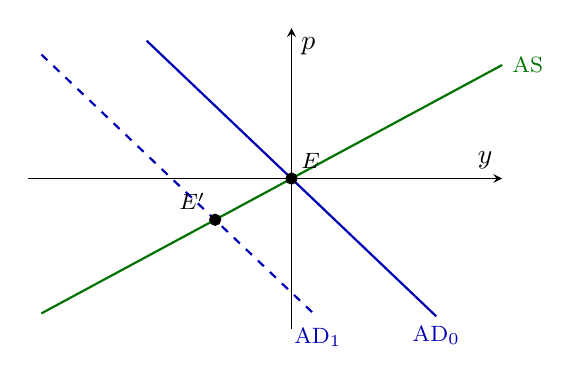
\begin{tikzpicture}
\begin{axis}[width=7.6cm,height=5.4cm,xmin=-1,xmax=0.8,ymin=-1.2,ymax=1.2,xlabel={$y$},ylabel={$p$},axis lines=middle,
  xtick=\empty,ytick=\empty,clip=false]
\addplot[green!45!black,thick,domain=-0.95:0.8] {1.133*x} node[right] {\footnotesize AS};
\addplot[blue!70!black,thick,domain=-0.55:0.55] {-2*x} node[below] {\footnotesize AD$_0$};
\addplot[blue!70!black,thick,dashed,domain=-0.95:0.1] {-2*(x+0.455)} node[below] {\footnotesize AD$_1$};
\addplot[only marks,mark=*] coordinates {(0,0) (-0.290,-0.329)};
\node[above right] at (axis cs:0,0) {\footnotesize $E$};
\node[above left] at (axis cs:-0.29,-0.329) {\footnotesize $E'$};
\end{axis}
\end{tikzpicture}
\end{center}
\passo{policy}{To restore $p=p^e$ and $y=y_n$, set $dp=dy=0$ in \eqref{b8:AD} differentiated with $di\neq0$:}
\begin{align*}
0&=d\bar y_n-\sigma\,di,\\
di&=\frac{d\bar y_n}{\sigma}\\
&=\frac{\big(-\frac{d\bar\tau}{\sigma^{-1}+\eta}\big)}{\sigma}\\
&=-\frac{d\bar\tau}{\sigma(\sigma^{-1}+\eta)}=-\frac{(1)}{0.5\times2.2}=-0.909 .
\end{align*}
Cut $i$ by $0.909$ points: AD returns to AD$_0$, so $y=y_n=y_e$ and $p=p^e$ together.
No trade-off: the shock is to demand and leaves $y_n=y_e$ (the divine coincidence, Block 9). Raising $i$ would deepen the fall.
\intuicao{Future taxes make households poorer in the long run, so they consume less now; with preset prices, output falls.}
\refbib{Benigno (2015), \S4, eq.~(13) (taxes in the markup); \S5, eqs.~(20)--(21); \S8, p.~514; Prova~01, Q3(a)--(b).}
\rubrica{\item $dy$, $dp$ and both gaps: 1.5 pts. \item Numbers: 0.5 pt. \item Graph: axes, AD shift left, AS fixed, $E'$: 1 pt.
\item Policy sign and no trade-off: 1 pt. Shifting the AS: max.\ 1 pt in the item. Raising $i$: 0 for the policy line.}
\end{sol}
